\documentclass[12pt,a4paper]{article}
% Packages
\usepackage[T1]{fontenc}
\usepackage[utf8]{inputenc}
\usepackage{lmodern}
\usepackage[a4paper,top=2.5cm,bottom=2.5cm,left=2.5cm,right=2.5cm]{geometry}
\usepackage{microtype}
\usepackage{parskip}
\usepackage{xcolor}
\usepackage{graphicx}
\usepackage{booktabs}
\usepackage{tabularx}
\usepackage{longtable}
\usepackage{array}
\usepackage{enumitem}
\usepackage{fancyhdr}
\usepackage{titlesec}
\usepackage{caption}
\usepackage{float}
\usepackage{hyperref}
\usepackage{listings}
\usepackage{tikz}
\definecolor{codebg}{HTML}{FFFDE7}
\definecolor{codeborder}{HTML}{DEE2E6}
\definecolor{codegreen}{HTML}{198754}
\definecolor{codepurple}{HTML}{6F42C1}
\definecolor{codeblue}{HTML}{0D6EFD}
\definecolor{codegray}{HTML}{6C757D}
\lstdefinelanguage{TypeScript}{
  keywords={const,let,var,function,async,await,return,if,else,throw,new,
            import,from,export,class,interface,type,try,catch,true,false,null},
  keywordstyle=\color{codeblue}\bfseries,
  ndkeywords={string,number,boolean,void,Promise},
  ndkeywordstyle=\color{codepurple},
  comment=[l]{//},
  morecomment=[s]{/*}{*/},
  commentstyle=\color{codegreen}\itshape,
  stringstyle=\color{codegreen},
  morestring=[b]',
  morestring=[b]",
  sensitive=true
}
\lstset{
  language=TypeScript,
  basicstyle=\ttfamily\footnotesize,
  backgroundcolor=\color{codebg},
  frame=single, framesep=4pt, rulecolor=\color{codeborder},
  breaklines=true, showstringspaces=false,
  tabsize=2, captionpos=b,
  numbers=left, numberstyle=\tiny\color{codegray}, numbersep=8pt,
  xleftmargin=2em, xrightmargin=6pt,
  aboveskip=0.6em, belowskip=0.4em,
}
\usetikzlibrary{arrows.meta,positioning,shapes.geometric,fit,backgrounds}
\hypersetup{
  colorlinks=true,
  linkcolor=black,
  urlcolor=blue,
  pdftitle={Architecture Design Documentation - Sarajevo Expats},
  pdfauthor={Sarajevo Expats Team}
}
\pagestyle{fancy}
\fancyhf{}
\setlength{\headheight}{14.5pt}
\fancyhead[L]{\small CS308 Software Engineering}
\fancyhead[R]{\small Architecture Design Documentation}
\fancyfoot[C]{\thepage}
\renewcommand{\headrulewidth}{0.4pt}
\renewcommand{\footrulewidth}{0.4pt}
\titleformat{\section}{\large\bfseries}{\thesection}{1em}{}
\titleformat{\subsection}{\normalsize\bfseries}{\thesubsection}{1em}{}
\titleformat{\subsubsection}{\normalsize\itshape}{\thesubsubsection}{1em}{}
\setlist[itemize]{leftmargin=2em}
\setlist[enumerate]{leftmargin=2em}
\renewcommand{\arraystretch}{1.25}
\captionsetup[table]{position=top,labelfont=bf,font=small,skip=0.45em}
\captionsetup[figure]{labelfont=bf,font=small}
\sloppy
\definecolor{IUSBlue}{HTML}{1E3A8A}
\definecolor{LayerBlue}{HTML}{DBEAFE}
\definecolor{LayerGreen}{HTML}{DCFCE7}
\definecolor{LayerOrange}{HTML}{FFEDD5}
\definecolor{LayerRed}{HTML}{FEE2E2}
\definecolor{LayerGray}{HTML}{F3F4F6}
\tikzset{
  archbox/.style={
    draw,
    rounded corners=4pt,
    align=center,
    font=\small,
    minimum height=1.0cm,
    inner xsep=8pt,
    inner ysep=6pt
  },
  layerbox/.style={
    draw,
    rounded corners=5pt,
    align=center,
    font=\small\bfseries,
    minimum width=12.2cm,
    minimum height=1.05cm,
    inner sep=6pt
  },
  smallbox/.style={
    draw,
    rounded corners=3pt,
    align=center,
    font=\footnotesize,
    minimum width=3.5cm,
    minimum height=0.75cm,
    fill=white
  },
  arrow/.style={-{Stealth[length=6pt]}, thick},
  dashedarrow/.style={-{Stealth[length=6pt]}, thick, dashed}
}
\newcommand{\decorativerule}{%
  \makebox[0.23\textwidth]{\hrulefill}%
  \hspace{0.8em}\textbullet\hspace{0.8em}%
  \makebox[0.23\textwidth]{\hrulefill}%
}
\makeatletter
\newcommand{\fancytableofcontents}{%
  \begin{center}
    {\Huge Contents}\\[-0.15em]
    \decorativerule
  \end{center}
  \vspace{1.2cm}
  \@starttoc{toc}
}
\makeatother
\begin{document}
\pagenumbering{gobble}
\begin{titlepage}
  \centering
  \vspace*{0.35cm}
  \IfFileExists{ius-logo.png}{%
    \includegraphics[width=2.85cm]{ius-logo.png}%
  }{%
    \includegraphics[width=2.85cm]{ius_logo.png}%
  }\\[1.55cm]
  {\Large\bfseries INTERNATIONAL UNIVERSITY OF SARAJEVO}\\[0.55em]
  {\large Faculty of Engineering and Natural Sciences}\\[0.55em]
  {\large Department of Computer Science and Engineering}\\[1.55cm]
  {\Huge\bfseries Architecture Design Documentation}\\[0.75em]
  {\Large\bfseries Sarajevo Expats}\\[0.45em]
  {\large Spring Semester 2025--2026}
  \vfill
  \begin{minipage}[t]{0.54\textwidth}
    \raggedright
    \textbf{Prepared by:}\\[0.45em]
    Fatih Bahadır Karakuş (220302370)\\[0.12em]
    Ömer Faruk Yaşar (220302323)\\[0.12em]
    Taylan Taşkın (220302443)\\[0.12em]
    Kayra Yılmaz (220302421)\\[0.12em]
    Ata Arda Kara (230302007)
  \end{minipage}%
  \hfill%
  \begin{minipage}[t]{0.40\textwidth}
    \raggedleft
    \textbf{Course:}\\[0.3em]
    CS308 Software Engineering\\[0.9em]
    \textbf{Instructor:}\\[0.3em]
    Mirza Selimović\\[0.9em]
    \textbf{Lab Assistant:}\\[0.3em]
    Adna Dedić
  \end{minipage}
  \vfill
  \rule{0.55\textwidth}{0.4pt}\\[0.55cm]
  {\normalsize Sarajevo, May 2026}
\end{titlepage}
\pagenumbering{roman}
\fancytableofcontents
\newpage
\pagenumbering{arabic}
\section{Introduction}
This document presents the architecture design of \textit{Sarajevo Expats}, a mobile-first
community platform developed for the CS308 Software Engineering project. The system
centralizes community news, event discovery, RSVP management, waitlist handling, global
chat, event-based chat rooms, and personal profile tracking for the Sarajevo expat
community.
The goal of this report is to explain and justify the main architectural decisions behind
the system. It covers the design patterns used or planned, the selected architecture style,
the architecture diagram, the interaction between major components, the data flow across
the system, and the security approach used for communication and authorization.
The documentation is based on the current project structure, the Software Requirements
Specification, and the System Diagrams Report. Where the implementation is still in the
MVP or mock-data stage, this report explicitly separates current implementation from
planned production behavior.
\section{Design Patterns}
\subsection{Overview}
The Sarajevo Expats system uses several architectural and design patterns to keep the
codebase modular, maintainable, and easier to extend. Some patterns are already visible
in the current implementation, while others are planned for the production version of the
system.
\begin{figure}[H]
\centering
\resizebox{0.96\textwidth}{!}{
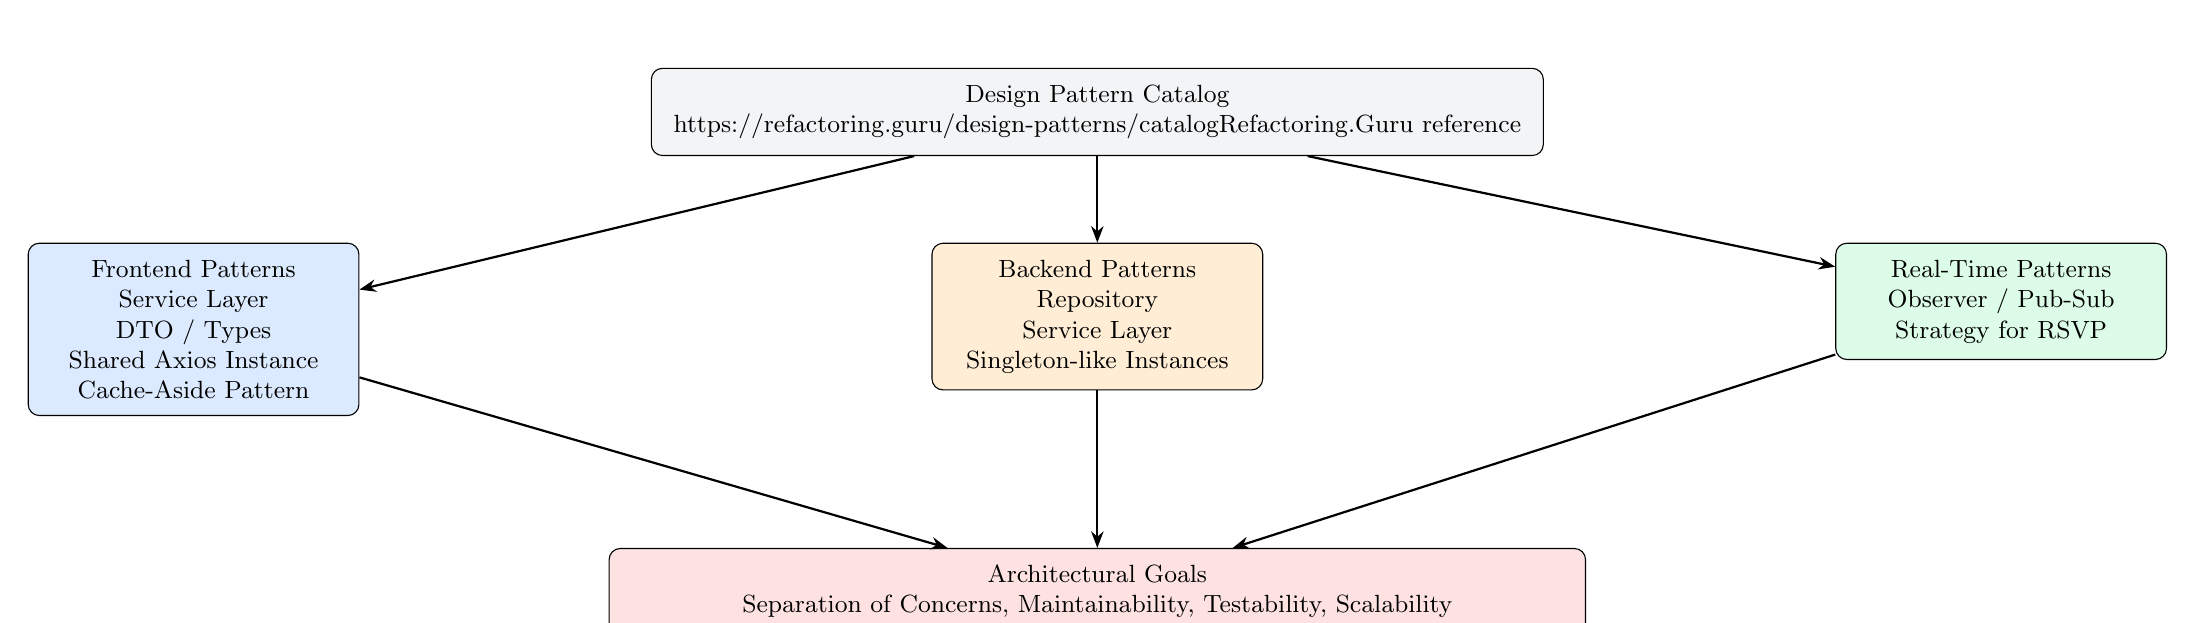
\begin{tikzpicture}[node distance=1.0cm]
  \node[archbox, fill=LayerGray, minimum width=4.5cm] (catalog)
    {Design Pattern Catalog\\\href{https://refactoring.guru/design-patterns/catalog}{Refactoring.Guru} reference};
  \node[archbox, fill=LayerBlue, below left=1.1cm and 3.7cm of catalog, minimum width=4.2cm] (frontend)
    {Frontend Patterns\\Service Layer\\DTO / Types\\Shared Axios Instance\\Cache-Aside Pattern};
  \node[archbox, fill=LayerOrange, below=1.1cm of catalog, minimum width=4.2cm] (backend)
    {Backend Patterns\\Repository\\Service Layer\\Singleton-like Instances};
  \node[archbox, fill=LayerGreen, below right=1.1cm and 3.7cm of catalog, minimum width=4.2cm] (realtime)
    {Real-Time Patterns\\Observer / Pub-Sub\\Strategy for RSVP};
  \node[archbox, fill=LayerRed, below=2.0cm of backend, minimum width=12.4cm] (outcome)
    {Architectural Goals\\Separation of Concerns, Maintainability, Testability, Scalability};
  \draw[arrow] (catalog) -- (frontend);
  \draw[arrow] (catalog) -- (backend);
  \draw[arrow] (catalog) -- (realtime);
  \draw[arrow] (frontend) -- (outcome);
  \draw[arrow] (backend) -- (outcome);
  \draw[arrow] (realtime) -- (outcome);
\end{tikzpicture}
}
\caption{Design pattern usage overview in Sarajevo Expats}
\end{figure}
\subsection{Repository Pattern}
\textbf{Where it appears:} \texttt{backend/src/repositories/eventRepository.ts} and \texttt{backend/src/repositories/chatRepository.ts}.
\textbf{Description:} The Repository Pattern separates data-access operations from
business logic. Controllers and services never import Mongoose directly; they call
repository methods and receive typed result objects. The repositories expose a clean
interface: \texttt{getAll()}, \texttt{getById()}, \texttt{create()},
\texttt{incrementRSVP()}, \texttt{addToWaitlist()}, \texttt{getMessagesByRoomId()},
and \texttt{saveMessage()}.
\textbf{Reason for use:} Decoupling services from the database engine means the storage
backend can be swapped or mocked in tests without touching any business logic.
\begin{lstlisting}[caption={eventRepository.ts -- getAll, getById, create, incrementRSVP, addToWaitlist}]
import { Event, IEvent } from '../models/Event';
import mongoose from 'mongoose';
export const eventRepository = {
  getAll: async (): Promise<IEvent[]> =>
    await Event.find().sort({ date: 1 }),
  getById: async (id: string): Promise<IEvent | null> => {
    if (!mongoose.Types.ObjectId.isValid(id)) return null;
    return await Event.findById(id);
  },
  create: async (data: Partial<IEvent>): Promise<IEvent> =>
    await Event.create(data),
  incrementRSVP: async (id: string, userId: string): Promise<IEvent | null> => {
    const event = await Event.findByIdAndUpdate(
      id,
      { $inc: { currentRSVP: 1 },
        $push: { participants: new mongoose.Types.ObjectId(userId) } },
      { new: true }
    );
    if (event) event.isFull = event.currentRSVP >= event.capacity;
    return event;
  },
  addToWaitlist: async (id: string, userId: string): Promise<IEvent | null> =>
    await Event.findByIdAndUpdate(
      id,
      { $addToSet: { waitlist: new mongoose.Types.ObjectId(userId) } },
      { new: true }
    ),
};
\end{lstlisting}
\begin{lstlisting}[caption={chatRepository.ts -- getMessagesByRoomId and saveMessage}]
import { Message, IMessage } from '../models/Message';
import mongoose from 'mongoose';
export const chatRepository = {
  getMessagesByRoomId: async (roomId: string): Promise<IMessage[]> =>
    await Message.find({ roomId, hidden: false }).sort({ createdAt: 1 }),
  saveMessage: async (data: {
    roomId: string;
    senderId: string;
    senderName: string;
    content: string;
  }): Promise<IMessage> => {
    const message = new Message({
      ...data,
      senderId: new mongoose.Types.ObjectId(data.senderId),
    });
    return await message.save();
  },
};
\end{lstlisting}
\subsection{Service Layer Pattern}
\textbf{Where it appears:} \texttt{src/services/authService.ts}, \texttt{src/services/eventService.ts}, \texttt{src/services/chatService.ts}, and \texttt{backend/src/services/eventService.ts}.
\textbf{Description:} The Service Layer Pattern places application-specific business logic
in dedicated service modules between route handlers and the repository layer. Controllers
remain thin — they parse HTTP input and delegate all domain logic to a service.
\textbf{Reason for use:} Business rules live in one place and can be reused from a REST
handler, a Socket.IO handler, or a future scheduled job without duplication.
\begin{lstlisting}[caption={eventService.ts -- business logic isolated from the route handler}]
export const eventService = {
  processRsvp: async (eventId: string, userId: string) => {
    const event = await eventRepository.getById(eventId);
    if (!event) throw new Error('Event not found');
    if (event.currentRSVP >= event.capacity) {
      // Capacity full: delegate to waitlist strategy
      await eventRepository.addToWaitlist(eventId, userId);
      return { status: 'waitlisted',
               message: `Added to waitlist for "${event.title}".` };
    }
    // Capacity available: confirm participation
    const updated = await eventRepository.incrementRSVP(eventId, userId);
    return { status: 'confirmed',
             message: `RSVP confirmed for "${updated?.title}".` };
  },
};
\end{lstlisting}
\subsection{Observer / Publish-Subscribe Pattern}
\textbf{Where it appears:} \texttt{backend/src/socket/chatHandler.ts}.
\textbf{Description:} Clients subscribe to a room via \texttt{join\_room}. When any
client emits \texttt{send\_message}, the server persists the message to MongoDB and
broadcasts \texttt{receive\_message} to every socket in that room with
\texttt{io.to(roomId).emit()}. No client polls the server --- they are notified instantly.
\textbf{Reason for use:} The publish-subscribe model eliminates polling, reduces
unnecessary network traffic, and delivers messages with minimal latency as required
by the real-time performance goal of the system.
\begin{lstlisting}[caption={chatHandler.ts -- Observer pattern via Socket.IO room broadcast}]
export const initializeChatSocket = (io: Server) => {
  io.on('connection', (socket: Socket) => {
    // Subscriber joins a room (subscribes to a channel)
    socket.on('join_room', async (roomId: string) => {
      socket.join(roomId);
      const history = await chatRepository.getMessagesByRoomId(roomId);
      socket.emit('previous_messages', history);
    });
    // Publisher sends a message -> server notifies all subscribers
    socket.on('send_message', async (data) => {
      const saved = await chatRepository.saveMessage(data);
      io.to(data.roomId).emit('receive_message', saved); // broadcast
    });
  });
};
\end{lstlisting}
\subsection{Singleton-Like Shared Instance Pattern}
\textbf{Where it appears:} \texttt{src/services/api.ts} (frontend Axios instance) and \texttt{backend/src/index.ts} (HTTP server, Socket.IO server, MongoDB connection).
\textbf{Description:} Critical runtime resources are created once at startup and shared
across the application. The frontend uses one configured Axios instance with base URL,
timeout, and JWT interceptors. The backend opens one MongoDB connection pool and one
Socket.IO server that all repositories and handlers reuse.
\textbf{Reason for use:} Opening a new database connection per request would exhaust
MongoDB Atlas connection limits and add significant latency. A single shared pool
handles concurrency efficiently without any duplication.
\begin{lstlisting}[caption={index.ts -- single MongoDB connection and Socket.IO instance}]
import mongoose from 'mongoose';
import { Server } from 'socket.io';
// One DB connection shared by all repositories
mongoose.connect(process.env.MONGO_URI!)
  .then(() => console.log('[DB] MongoDB connected'))
  .catch(err => { console.error(err); process.exit(1); });
// One HTTP server and one Socket.IO instance for the entire runtime
const server = http.createServer(app);
const io = new Server(server, { cors: { origin: config.cors.origins } });
initializeChatSocket(io); // same io passed to all socket handlers
\end{lstlisting}
\begin{lstlisting}[caption={api.ts -- single Axios instance shared by all client services}]
const api: AxiosInstance = axios.create({
  baseURL: BASE_URL,
  timeout: 10000,
});
// Attach JWT to every outgoing request automatically
api.interceptors.request.use(async (config) => {
  const token = await AsyncStorage.getItem('auth_token');
  if (token) config.headers.Authorization = `Bearer ${token}`;
  return config;
});
export default api; // imported by authService, eventService, chatService...
\end{lstlisting}
\subsection{DTO and Type Definition Pattern}
\textbf{Where it appears:} \texttt{src/types/user.types.ts}, \texttt{src/types/event.types.ts}, and \texttt{src/types/news.types.ts}.
\textbf{Description:} TypeScript interfaces define the exact shape of data that crosses
layer boundaries. Examples include \texttt{LoginRequest}, \texttt{LoginResponse},
\texttt{RegisterRequest}, \texttt{JwtPayload}, \texttt{User}, \texttt{Event}, and
\texttt{News}. These types are shared between the frontend service layer and the backend
route handlers.
\textbf{Reason for use:} Typed contracts make API integration mistakes visible at compile
time rather than at runtime. They also serve as living documentation --- any developer can
read the interface and know exactly what a request or response looks like.
\begin{lstlisting}[caption={user.types.ts -- LoginRequest, LoginResponse, RegisterRequest, JwtPayload}]
export interface LoginRequest {
  email: string;
  password: string;
}
export interface RegisterRequest {
  username: string;
  email: string;
  password: string;
  phone?: string;
}
export interface LoginResponse {
  token: string;
  user: { id: string; username: string; email: string; type: string };
}
export interface JwtPayload {
  id: string;
  type: 'member' | 'GM';
  iat: number;
  exp: number;
}
\end{lstlisting}
\begin{lstlisting}[caption={event.types.ts and news.types.ts -- User, Event, News DTOs}]
// user.types.ts
export interface User {
  id: string;
  username: string;
  email: string;
  type: 'member' | 'GM';
  interests: string[];
  attendedEvents: string[];
}
// event.types.ts
export interface Event {
  id: string;
  title: string;
  description: string;
  location: string;
  date: string;
  category: string;
  capacity: number;
  currentRSVP: number;
  isFull: boolean;
}
// news.types.ts
export interface News {
  id: string;
  title: string;
  content: string;
  imageUrl?: string;
  publishedAt: string;
}
\end{lstlisting}
\subsection{Strategy Pattern for RSVP Handling}
\textbf{Status:} Planned and partially represented by the current conditional RSVP logic.
\textbf{Where it applies:} RSVP behavior in \texttt{backend/src/services/eventService.ts}.
\textbf{Description:} The RSVP flow has two possible behaviors: direct join when an
event has available capacity, and waitlist placement when the event is full. Both
behaviors are triggered through the same \texttt{processRsvp()} entry point.
\textbf{Reason for use:} In the production version, these behaviors can be formalized as
separate strategies such as \texttt{DirectJoinStrategy} and \texttt{WaitlistStrategy}.
This would keep the RSVP service extensible if the team later adds priority waitlists,
organizer approval, paid events, or cancellation-based promotion from waitlist to
confirmed attendee.

% ---------------------------------------------------------------
% NEW SECTION 2.8 — Cache-Aside / Stale-While-Revalidate Pattern
% ---------------------------------------------------------------
\subsection{Cache-Aside / Stale-While-Revalidate Pattern}
\textbf{Where it appears:} \texttt{src/services/storageService.ts} and the
\texttt{useCachedFetch} hook exported from the same file.
\textbf{Description:} The mobile client applies a cache-aside strategy backed by
AsyncStorage. Every data type has its own TTL: events are cached for 5 minutes,
places and news for 10 minutes, and chat messages for 2 minutes. When a screen
opens, the client checks the cache first. If a valid, non-expired entry exists it is
shown immediately without a network request. If the entry is stale the screen still
renders the cached data instantly while a background fetch retrieves fresh data and
updates the cache. If there is no internet connection at all, the last-known cached
value is shown as an offline fallback. The \texttt{useCachedFetch} hook encapsulates
this logic so every screen in the application can use it with a single call.
\textbf{Reason for use:} React Native apps on mobile networks can experience slow or
intermittent connectivity. Showing cached data immediately removes perceived loading
time for the user, while background refresh keeps the content up to date. The
pattern also reduces the number of round trips to the backend, which lowers server
load and prevents unnecessary JWT-authenticated requests.
\begin{lstlisting}[caption={storageService.ts -- TTL cache, stale-while-revalidate, and offline fallback}]
const TTL: Record<string, number> = {
  events:        5 * 60 * 1000,   // 5 minutes
  places:       10 * 60 * 1000,   // 10 minutes
  news:         10 * 60 * 1000,
  chat_messages: 2 * 60 * 1000,   // 2 minutes
};
export const storageService = {
  async set<T>(key: string, data: T): Promise<void> {
    const entry = { data, savedAt: Date.now() };
    await AsyncStorage.setItem(`cache_${key}`, JSON.stringify(entry));
  },
  // Returns null when the entry is expired
  async get<T>(key: string): Promise<T | null> {
    const raw = await AsyncStorage.getItem(`cache_${key}`);
    if (!raw) return null;
    const entry = JSON.parse(raw);
    const ttl = TTL[key] ?? TTL['places'];
    return Date.now() - entry.savedAt > ttl ? null : entry.data;
  },
  // Returns stale data regardless of TTL (offline fallback)
  async getStale<T>(key: string): Promise<T | null> {
    const raw = await AsyncStorage.getItem(`cache_${key}`);
    return raw ? JSON.parse(raw).data : null;
  },
};
// Hook used by every screen:
// const { data, loading, refresh } = useCachedFetch('events', eventService.getAll);
export function useCachedFetch<T>(key: string, fetcher: () => Promise<T>) {
  const [data, setData] = useState<T | null>(null);
  const load = useCallback(async (forceRefresh = false) => {
    if (!forceRefresh) {
      const cached = await storageService.getStale<T>(key);
      if (cached) {
        setData(cached);
        const stale = await storageService.isStale(key);
        if (!stale) return;           // still fresh, skip network
      }
    }
    const fresh = await fetcher();    // background or forced fetch
    setData(fresh);
    await storageService.set(key, fresh);
  }, [key]);
  useEffect(() => { load(); }, [load]);
  return { data, refresh: () => load(true) };
}
\end{lstlisting}

\subsection{Pattern Interactions}
The design patterns used in Sarajevo Expats do not operate in isolation. Each pattern
depends on or enables at least one other pattern, forming a layered chain where
higher-level patterns are only possible because lower-level ones are already in place.
\begin{figure}[H]
\centering
\resizebox{0.94\textwidth}{!}{
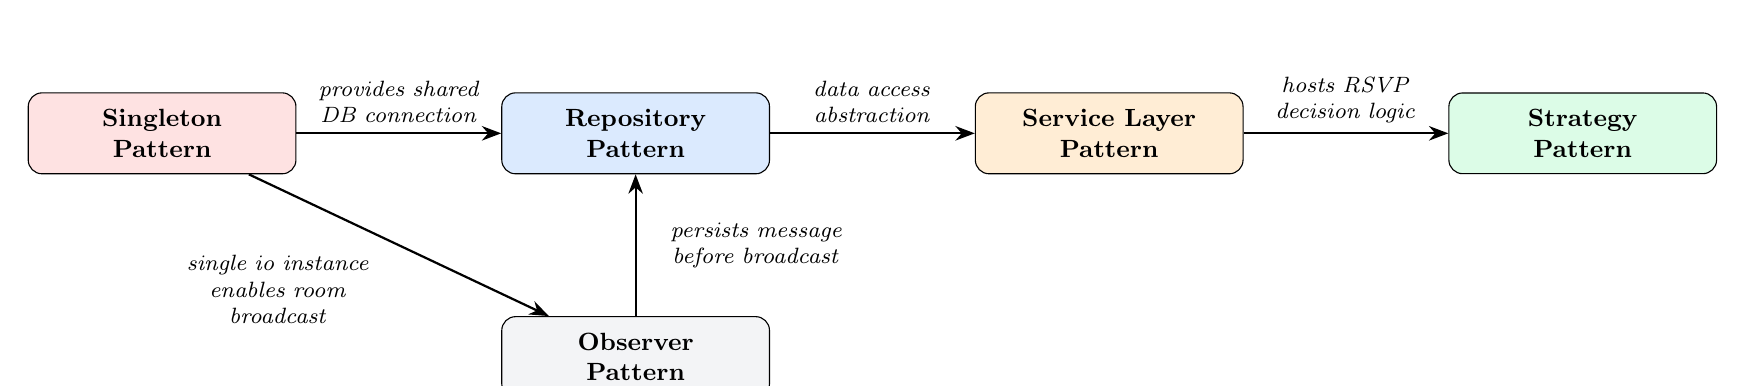
\begin{tikzpicture}[
  node distance=1.4cm and 2.6cm,
  patbox/.style={
    draw, rounded corners=5pt, align=center,
    font=\small\bfseries, minimum width=3.4cm, minimum height=1.0cm,
    inner sep=6pt
  },
  rel/.style={-{Stealth[length=7pt]}, thick},
  lbl/.style={font=\footnotesize\itshape, text width=2.6cm, align=center}
]
\node[patbox, fill=LayerRed]    (singleton) {Singleton\\Pattern};
\node[patbox, fill=LayerBlue,   right=of singleton] (repository) {Repository\\Pattern};
\node[patbox, fill=LayerOrange, right=of repository] (service) {Service Layer\\Pattern};
\node[patbox, fill=LayerGreen,  right=of service] (strategy) {Strategy\\Pattern};
\node[patbox, fill=LayerGray,   below=1.8cm of repository] (observer) {Observer\\Pattern};
% Singleton -> Repository
\draw[rel] (singleton) -- node[above, lbl] {provides shared\\DB connection} (repository);
% Repository -> Service Layer
\draw[rel] (repository) -- node[above, lbl] {data access\\abstraction} (service);
% Service Layer -> Strategy
\draw[rel] (service) -- node[above, lbl] {hosts RSVP\\decision logic} (strategy);
% Observer -> Repository
\draw[rel] (observer) -- node[right, lbl, text width=2.8cm] {persists message\\before broadcast} (repository);
% Singleton -> Observer
\draw[rel] (singleton) -- node[below left, lbl, text width=2.8cm] {single io instance\\enables room broadcast} (observer);
\end{tikzpicture}
}
\caption{Relationships between design patterns in Sarajevo Expats}
\end{figure}
The five patterns form two interacting chains. The first chain runs horizontally:
\textbf{Singleton} provides the single shared MongoDB connection that all
\textbf{Repository} instances rely on. The Repository abstraction is what allows the
\textbf{Service Layer} to apply business logic without knowing anything about the
database. The Strategy pattern for RSVP handling lives entirely inside the Service
Layer, so it is only possible because the service and repository layers beneath it are
already in place.
The second chain involves the \textbf{Observer} pattern. When a chat message arrives
via Socket.IO, the Observer cannot safely broadcast to room subscribers until the message
has been persisted. It therefore calls the \textbf{Repository} before emitting
\texttt{receive\_message}. At the same time, the Observer's broadcast capability depends
on there being a single shared Socket.IO server instance --- which is the \textbf{Singleton}
pattern applied to the \texttt{io} object in \texttt{backend/src/index.ts}. If multiple
\texttt{io} instances existed, sockets in the same room could be spread across different
server objects and would never receive each other's messages.
In summary, removing any one pattern from the system would either break or significantly
degrade the patterns that depend on it. This interdependency is intentional: each pattern
was chosen not only for its own benefits but also because it enables the patterns above
it in the chain.
\section{Chosen Architecture Style}
\subsection{Selected Style}
The selected architecture style is a \textbf{Layered Client-Server Architecture}.
The system has one mobile client that communicates with a centralized backend server.
Inside the server side, responsibilities are separated into layers: routes/controllers,
services, repositories, and database storage. The real-time chat feature is added as an
event-driven communication subsystem using Socket.IO.
In one sentence, the system can be described as follows:
\begin{quote}
\textit{Sarajevo Expats uses a client-server architecture, with a layered backend and an
event-driven real-time messaging subsystem.}
\end{quote}
\subsection{Architecture Diagram}
\begin{figure}[H]
\centering
\resizebox{\textwidth}{!}{
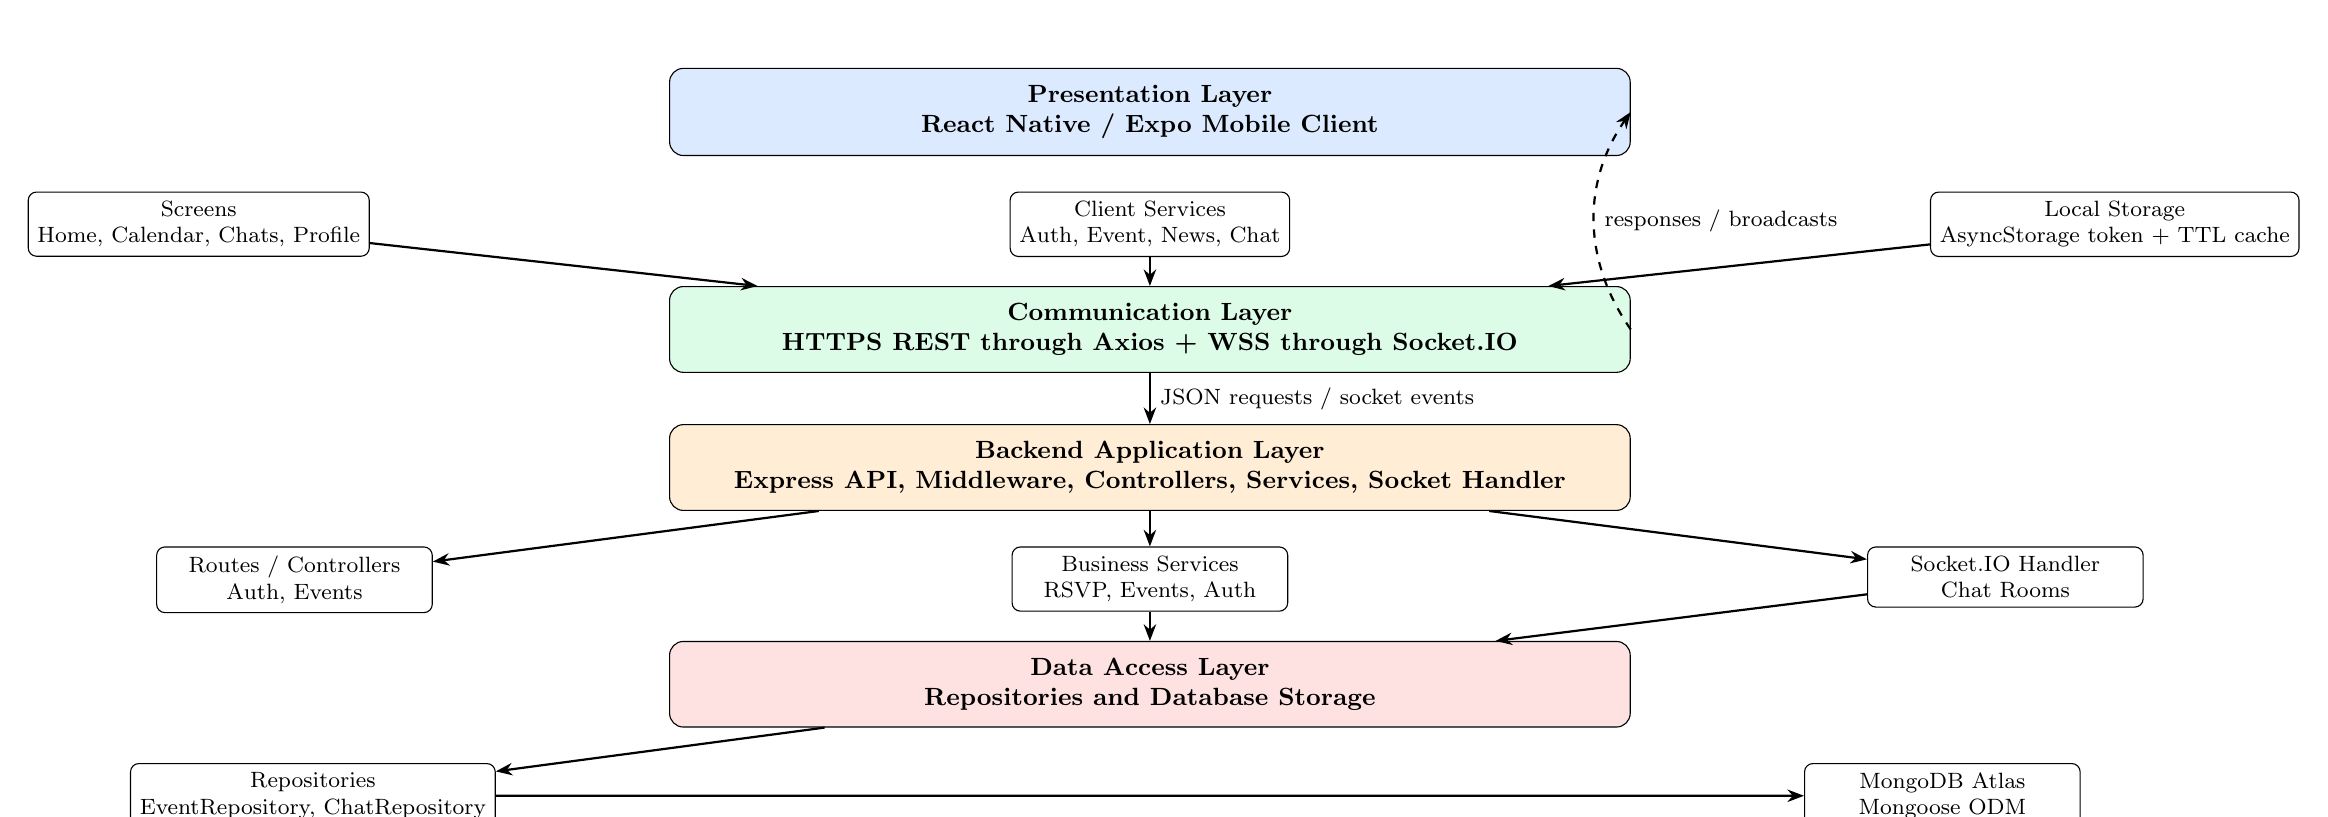
\begin{tikzpicture}[node distance=0.55cm]
  \node[layerbox, fill=LayerBlue] (presentation)
    {Presentation Layer\\React Native / Expo Mobile Client};
  \node[smallbox, below left=0.45cm and 3.8cm of presentation] (screens)
    {Screens\\Home, Calendar, Chats, Profile};
  \node[smallbox, below=0.45cm of presentation] (clientservices)
    {Client Services\\Auth, Event, News, Chat};
  \node[smallbox, below right=0.45cm and 3.8cm of presentation] (storage)
    {Local Storage\\AsyncStorage token + TTL cache};
  \node[layerbox, fill=LayerGreen, below=1.65cm of presentation] (communication)
    {Communication Layer\\HTTPS REST through Axios + WSS through Socket.IO};
  \node[layerbox, fill=LayerOrange, below=0.65cm of communication] (backend)
    {Backend Application Layer\\Express API, Middleware, Controllers, Services, Socket Handler};
  \node[smallbox, below left=0.45cm and 3.0cm of backend] (routes)
    {Routes / Controllers\\Auth, Events};
  \node[smallbox, below=0.45cm of backend] (services)
    {Business Services\\RSVP, Events, Auth};
  \node[smallbox, below right=0.45cm and 3.0cm of backend] (socket)
    {Socket.IO Handler\\Chat Rooms};
  \node[layerbox, fill=LayerRed, below=1.65cm of backend] (data)
    {Data Access Layer\\Repositories and Database Storage};
  \node[smallbox, below left=0.45cm and 2.2cm of data] (repositories)
    {Repositories\\EventRepository, ChatRepository};
  \node[smallbox, below right=0.45cm and 2.2cm of data] (database)
    {MongoDB Atlas\\Mongoose ODM};
  \draw[arrow] (screens) -- (communication);
  \draw[arrow] (clientservices) -- (communication);
  \draw[arrow] (storage) -- (communication);
  \draw[arrow] (communication) -- node[right,font=\footnotesize] {JSON requests / socket events} (backend);
  \draw[arrow] (backend) -- (routes);
  \draw[arrow] (backend) -- (services);
  \draw[arrow] (backend) -- (socket);
  \draw[arrow] (services) -- (data);
  \draw[arrow] (socket) -- (data);
  \draw[arrow] (data) -- (repositories);
  \draw[arrow] (repositories) -- (database);
  \draw[dashedarrow] (communication.east) to[bend left=35]
    node[right,font=\footnotesize] {responses / broadcasts} (presentation.east);
\end{tikzpicture}
}
\caption{High-level architecture diagram of Sarajevo Expats}
\end{figure}
\subsection{Layer Responsibilities}
\begin{longtable}{@{}p{0.25\textwidth}p{0.68\textwidth}@{}}
\caption{Layer responsibilities in the selected architecture}\\
\toprule
\textbf{Layer} & \textbf{Responsibility} \\
\midrule
\endhead
Presentation Layer &
The React Native and Expo mobile client renders screens, collects user input, manages
navigation, and displays data. It includes Home, Calendar, Chats, Event Detail, Profile,
Settings, Authentication, and related components. \\
\addlinespace
Communication Layer &
This layer connects the mobile client with the backend. Axios is used for REST API
communication, while Socket.IO is used for real-time chat. Payloads are JSON-based in
both channels. \\
\addlinespace
Business Logic Layer &
The Express backend receives requests, applies middleware, dispatches routes, executes
service-layer logic, and handles Socket.IO events. Event capacity checks, RSVP behavior,
chat-room joins, and message persistence are handled here. \\
\addlinespace
Data Access Layer &
Repository modules abstract all persistence operations. Mongoose models (\texttt{User},
\texttt{Event}, \texttt{Message}) define MongoDB document schemas. Repositories are
the only layer that imports Mongoose directly; all other layers call repository methods. \\
\bottomrule
\end{longtable}
\subsection{Why This Architecture Fits}
This architecture fits the project for several reasons. First, Sarajevo Expats is a
mobile-first system where a React Native client communicates with a backend API, so a
client-server style is the natural choice. Second, the system has clearly separable
responsibilities: UI rendering, API communication, business rules, and data persistence.
A layered structure makes these responsibilities explicit.
The architecture also matches the project scale. A microservices architecture would add
deployment, networking, monitoring, and service-discovery complexity that is unnecessary
for this academic MVP. A layered monolithic backend is easier for the team to build,
test, explain, and deploy while still keeping the internal structure clean.
Finally, the chat feature requires real-time bidirectional communication. Adding
Socket.IO to the backend allows the project to support chat rooms and message
broadcasting without changing the overall client-server design.
\section{Architecture Communication and Interaction}
\subsection{Communication Overview}
The system uses two main communication mechanisms:
\begin{table}[H]
\centering
\caption{Main communication channels}
\begin{tabularx}{\textwidth}{@{}l l X@{}}
\toprule
\textbf{Channel} & \textbf{Protocol} & \textbf{Used For} \\
\midrule
REST API & HTTPS + JSON & Authentication, event listing, event details, RSVP, news, profile data \\
Real-time chat & WSS + Socket.IO events & Global chat, event chat rooms, message broadcasting \\
\bottomrule
\end{tabularx}
\end{table}
\subsection{REST Request-Response Flow}
Standard application actions use a REST request-response model. The mobile client calls
service modules, service modules call the Axios API instance, and the backend processes
the request through routes, controllers, services, repositories, and storage.
\textbf{Example login flow:}
\begin{enumerate}
  \item The user enters email and password on the authentication screen.
  \item The mobile client sends a JSON request to the backend login endpoint.
  \item The backend validates the credentials with bcrypt and returns a signed JWT.
  \item The client stores the token in AsyncStorage for subsequent requests.
  \item If credentials are invalid the backend returns \texttt{401 Unauthorized}.
\end{enumerate}
\begin{lstlisting}[caption={authRoutes.ts -- real bcrypt + JWT login handler}]
router.post('/login', async (req, res) => {
  const { email, password } = req.body;
  const user = await User.findOne({ email });
  if (!user) return res.status(401).json({ message: 'Invalid credentials' });
  const match = await bcrypt.compare(password, user.password);
  if (!match) return res.status(401).json({ message: 'Invalid credentials' });
  const token = jwt.sign(
    { id: user._id, type: user.type },
    config.jwt.secret,
    { expiresIn: config.jwt.expiresIn }   // '7d'
  );
  res.status(200).json({ token, user: { id: user._id, username: user.username } });
});
\end{lstlisting}
\textbf{Example RSVP flow:}
\begin{enumerate}
  \item The user opens an event detail screen and taps the join button.
  \item The client sends a request to \texttt{POST /api/events/:id/rsvp}.
  \item The backend service checks the current RSVP count against the event capacity.
  \item If capacity is available, the user is added as a participant.
  \item If the event is full, the user is placed on a waitlist in the planned production flow.
  \item The backend returns a success or waitlist response, and the UI updates accordingly.
\end{enumerate}
\subsection{Real-Time Socket.IO Flow}
Chat uses Socket.IO because messages need to be delivered immediately to all users in a
room. The interaction is event-driven rather than request-response.
\begin{enumerate}
  \item The client opens a chat screen and emits \texttt{join\_room} with a room ID.
  \item The server adds the socket to that room.
  \item The server fetches previous messages using \texttt{ChatRepository}.
  \item The server emits \texttt{previous\_messages} back to the joining client.
  \item When a user sends a message, the client emits \texttt{send\_message}.
  \item The server saves the message and emits \texttt{receive\_message} to all clients in the room.
\end{enumerate}
\subsection{Message and Data Formats}
All REST payloads are JSON. A login request contains credentials, and successful login
responses contain authentication information. Event endpoints return event objects with
fields such as ID, title/content, date or timestamp, capacity, and related metadata.
Socket.IO message payloads are also JSON-based. A chat message contains:
\begin{table}[H]
\centering
\caption{Socket.IO chat message format}
\begin{tabularx}{0.86\textwidth}{@{}l X@{}}
\toprule
\textbf{Field} & \textbf{Meaning} \\
\midrule
\texttt{roomId} & The global, event, or direct-message room receiving the message \\
\texttt{senderId} & The unique identifier of the sender \\
\texttt{senderName} & The display name of the sender \\
\texttt{content} & The message text \\
\texttt{createdAt} & Server-generated timestamp \\
\texttt{hidden} & Planned moderation flag for unsafe content \\
\bottomrule
\end{tabularx}
\end{table}
\subsection{Component Dependencies}
\begin{table}[H]
\centering
\caption{Main component dependencies}
\begin{tabularx}{\textwidth}{@{}l X@{}}
\toprule
\textbf{Component} & \textbf{Depends On} \\
\midrule
Mobile screens & Client service modules, theme context, local UI state \\
Client services & Axios API client, Socket.IO client, AsyncStorage token + TTL cache \\
Axios API client & Environment-based API URL and request/response interceptors \\
Express app & Middleware, route modules, controllers \\
Event controller & Backend event service \\
Event service & Event repository \\
Socket handler & Socket.IO server and chat repository \\
Repositories & Mongoose models (User, Event, Message) and MongoDB Atlas \\
\bottomrule
\end{tabularx}
\end{table}
\section{Security in Communication}
\subsection{Who Can Send Requests?}
Authentication is based on JSON Web Tokens. After a successful login the backend signs
and returns a JWT containing the user's ID and role. The mobile client stores this token
in AsyncStorage and the shared Axios instance attaches it to every outgoing request via
the \texttt{Authorization: Bearer <token>} header. On the backend, a JWT middleware
layer verifies the token before any protected route handler is reached. Requests with a
missing, expired, or tampered token are rejected with \texttt{401 Unauthorized}.
\begin{lstlisting}[caption={authMiddleware.ts -- JWT verification before protected routes}]
import jwt from 'jsonwebtoken';
import { config } from '../config';
export const authenticate = (req: any, res: any, next: any) => {
  const header = req.headers.authorization;
  if (!header?.startsWith('Bearer '))
    return res.status(401).json({ message: 'No token provided' });
  try {
    const payload = jwt.verify(header.split(' ')[1], config.jwt.secret);
    req.user = payload; // { id, type } available to all downstream handlers
    next();
  } catch {
    res.status(401).json({ message: 'Invalid or expired token' });
  }
};
// Usage: router.post('/events', authenticate, requireRole('GM'), createEvent);
\end{lstlisting}
\subsection{What Actions Are Allowed?}
Authorization is role-based. The SRS and class diagram define user roles such as guest,
member, GM, and admin/moderator. The production authorization model is:
\begin{table}[H]
\centering
\caption{Role-based authorization model}
\begin{tabularx}{\textwidth}{@{}l X@{}}
\toprule
\textbf{Role} & \textbf{Allowed Actions} \\
\midrule
Guest & Register, log in, and view public entry points only \\
Member & Browse news, view events, RSVP, join allowed chat rooms, manage own profile \\
GM / Organizer & Create and manage events, inspect participant lists, coordinate event chat \\
Admin / Moderator & Moderate chat, manage users, review flagged messages, publish important updates \\
\bottomrule
\end{tabularx}
\end{table}
In practice, backend middleware should decode the JWT, attach the authenticated user to
the request context, and check the user's role before allowing protected actions. For
example, \texttt{POST /api/events} should require the GM or admin role, while
\texttt{POST /api/events/:id/rsvp} should require an authenticated member.
\subsection{How Data Is Protected in Transit}
In production, all REST communication should use HTTPS, and Socket.IO should use WSS
over TLS. This protects credentials, JWT tokens, profile data, RSVP actions, and chat
messages from being read or modified in transit.
Additional security mechanisms are included or planned:
\begin{itemize}
  \item \textbf{Helmet:} The backend uses Helmet to set safer HTTP headers.
  \item \textbf{CORS:} The backend uses CORS; production configuration should restrict allowed origins instead of accepting all origins.
  \item \textbf{Rate limiting:} API routes are rate-limited to reduce brute-force login attempts and request flooding.
  \item \textbf{Password hashing:} Production authentication should store passwords with bcrypt, never as plain text.
  \item \textbf{Input validation:} Login, register, event creation, RSVP, and chat-message payloads should be validated and sanitized before processing.
  \item \textbf{Socket authentication:} Socket.IO connections pass the JWT during the handshake so the server can reject unauthenticated clients.
  \item \textbf{Room authorization:} Users should only join event chat rooms for events they are allowed to access.
  \item \textbf{Moderation:} The planned AI moderation flow can flag unsafe chat messages and store them with a hidden or moderated status for auditability.
\end{itemize}
\subsection{Current Implementation and Planned Hardening}
\begin{table}[H]
\centering
\caption{Current implementation and planned production hardening}
\begin{tabularx}{\textwidth}{@{}l X X@{}}
\toprule
\textbf{Area} & \textbf{Currently Present} & \textbf{Planned / Required for Production} \\
\midrule
Client auth handling &
  Token storage, Authorization header injection in Axios, and login
  requests consolidated to \texttt{/api/users/login} &
  Full role-based route guards aligned with production backend \\
Backend API protection &
  Helmet, CORS, JSON parsing, request logging, rate limiting &
  JWT middleware and role-based route guards on all protected endpoints \\
Password security &
  Mock login route in MVP &
  bcrypt hashing and secure credential verification \\
Chat transport &
  Socket.IO room events, broadcast flow, and JWT token passed in
  socket handshake \texttt{auth} field (\texttt{socketService.ts}) &
  Server-side handshake token validation and room access checks \\
Data storage &
  Mock and in-memory repositories &
  MongoDB persistence with indexed collections \\
\bottomrule
\end{tabularx}
\end{table}
\section{Architecture Trade-Offs}
The selected architecture intentionally avoids microservices. While microservices can
provide independent deployment and scaling, they would introduce unnecessary complexity
for the current scope. The project is an academic MVP with one mobile client, one
backend, and a limited number of functional domains. A layered client-server design
provides enough separation while remaining understandable and maintainable for the
team.
The main trade-off is that the backend is still a single deployable unit. If the user base
grows significantly, the team could later split real-time messaging, event management,
or notification processing into separate services. The current architecture does not block
that evolution because domain logic is already separated into services and repositories.
\section{Conclusion}
Sarajevo Expats uses a layered client-server architecture supported by event-driven
real-time communication. The React Native mobile client handles presentation and user
interaction, Axios and Socket.IO handle communication, the Express backend handles
business logic and routing, and repositories isolate data access from the rest of the
system.
The selected architecture fits the project because it is simple enough for the MVP,
structured enough for maintainability, and flexible enough to support future production
requirements such as MongoDB persistence, JWT middleware, role-based access control,
authenticated Socket.IO connections, waitlist automation, and moderation workflows.
\section{References}
\begin{enumerate}
  \item Refactoring.Guru, \textit{Design Patterns Catalog}. Available at:
  \url{https://refactoring.guru/design-patterns/catalog}
  \item Sarajevo Expats project team, \textit{Software Requirements Specification for Sarajevo Expats}, CS308 Software Engineering, 2026.
  \item Sarajevo Expats project team, \textit{System Diagrams Report for Sarajevo Expats}, CS308 Software Engineering, 2026.
  \item Existing Sarajevo Expats TypeScript codebase, including the React Native mobile client and Express / Socket.IO backend.
\end{enumerate}
\appendix
\section{Abbreviations}
\begin{table}[H]
\centering
\caption{Abbreviations used in this document}
\begin{tabular}{@{}ll@{}}
\toprule
\textbf{Abbreviation} & \textbf{Meaning} \\
\midrule
API & Application Programming Interface \\
CORS & Cross-Origin Resource Sharing \\
DTO & Data Transfer Object \\
GM & General Manager / Organizer role \\
HTTPS & Hypertext Transfer Protocol Secure \\
JWT & JSON Web Token \\
MVP & Minimum Viable Product \\
REST & Representational State Transfer \\
SRS & Software Requirements Specification \\
TLS & Transport Layer Security \\
TTL & Time To Live (cache expiry duration) \\
WSS & WebSocket Secure \\
\bottomrule
\end{tabular}
\end{table}
\section{Referenced Project Files}
\begin{itemize}
  \item \texttt{src/services/api.ts}
  \item \texttt{src/services/authService.ts}
  \item \texttt{src/services/eventService.ts}
  \item \texttt{src/services/newsService.ts}
  \item \texttt{src/services/chatService.ts}
  \item \texttt{src/services/storageService.ts}
  \item \texttt{src/services/socketService.ts}
  \item \texttt{src/types/user.types.ts}
  \item \texttt{backend/src/app.ts}
  \item \texttt{backend/src/index.ts}
  \item \texttt{backend/src/controllers/eventController.ts}
  \item \texttt{backend/src/services/eventService.ts}
  \item \texttt{backend/src/repositories/eventRepository.ts}
  \item \texttt{backend/src/repositories/chatRepository.ts}
  \item \texttt{backend/src/socket/chatHandler.ts}
\end{itemize}
\end{document}
